\documentclass{standalone}
\usepackage{tikz}
\usetikzlibrary{patterns, positioning}


\begin{document}
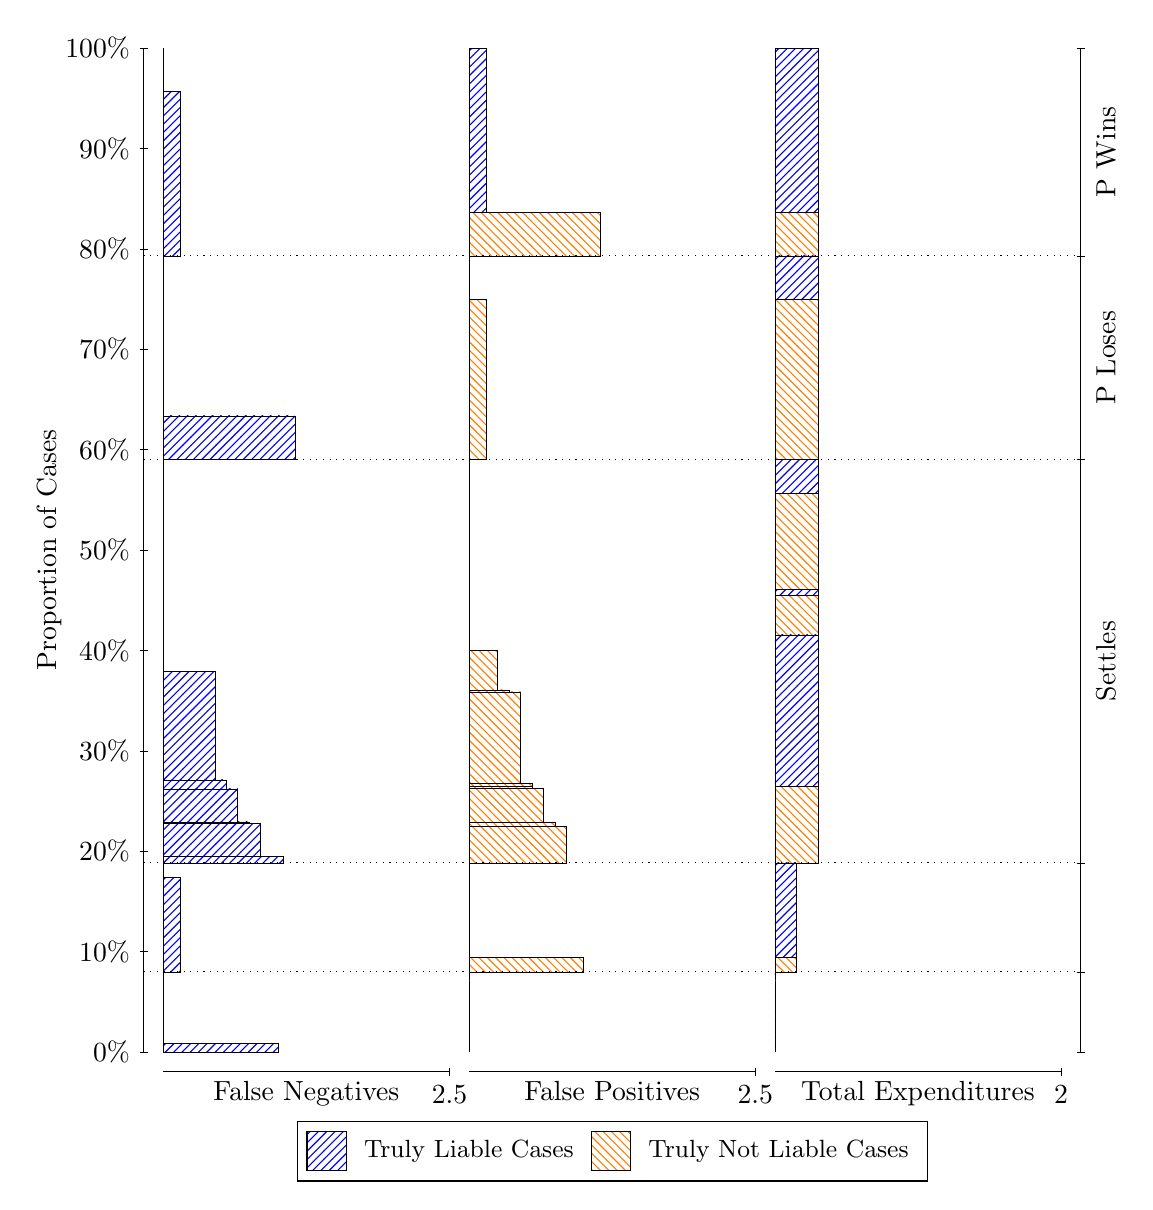
\begin{tikzpicture}
\draw[black, very thin] (1.5,1.75) -- (1.5,14.5);
\node[rotate=90, text=black, anchor=center] at (0.3, 8.125) {Proportion of Cases};
\draw[black, very thin] (1.45,1.75) -- (1.55,1.75);
\node[text=black, anchor=east] at (1.45, 1.75) {0\%};
\draw[black, very thin] (1.45,3.025) -- (1.55,3.025);
\node[text=black, anchor=east] at (1.45, 3.025) {10\%};
\draw[black, very thin] (1.45,4.3) -- (1.55,4.3);
\node[text=black, anchor=east] at (1.45, 4.3) {20\%};
\draw[black, very thin] (1.45,5.575) -- (1.55,5.575);
\node[text=black, anchor=east] at (1.45, 5.575) {30\%};
\draw[black, very thin] (1.45,6.85) -- (1.55,6.85);
\node[text=black, anchor=east] at (1.45, 6.85) {40\%};
\draw[black, very thin] (1.45,8.125) -- (1.55,8.125);
\node[text=black, anchor=east] at (1.45, 8.125) {50\%};
\draw[black, very thin] (1.45,9.4) -- (1.55,9.4);
\node[text=black, anchor=east] at (1.45, 9.4) {60\%};
\draw[black, very thin] (1.45,10.675) -- (1.55,10.675);
\node[text=black, anchor=east] at (1.45, 10.675) {70\%};
\draw[black, very thin] (1.45,11.95) -- (1.55,11.95);
\node[text=black, anchor=east] at (1.45, 11.95) {80\%};
\draw[black, very thin] (1.45,13.225) -- (1.55,13.225);
\node[text=black, anchor=east] at (1.45, 13.225) {90\%};
\draw[black, very thin] (1.45,14.5) -- (1.55,14.5);
\node[text=black, anchor=east] at (1.45, 14.5) {100\%};

\draw[black, very thin] (13.4,1.75) -- (13.4,14.5);
\draw[black, very thin] (13.35,1.75) -- (13.45,1.75);
\node[anchor=west] at (13.35, 1.75) {};
\draw[black, very thin] (13.35,2.7667) -- (13.45,2.7667);
\node[anchor=west] at (13.35, 2.7667) {};
\draw[black, very thin] (13.35,4.152) -- (13.45,4.152);
\node[anchor=west] at (13.35, 4.152) {};
\draw[black, very thin] (13.35,9.2757) -- (13.45,9.2757);
\node[anchor=west] at (13.35, 9.2757) {};
\draw[black, very thin] (13.35,11.861) -- (13.45,11.861);
\node[anchor=west] at (13.35, 11.861) {};
\draw[black, very thin] (13.35,14.5) -- (13.45,14.5);
\node[anchor=west] at (13.35, 14.5) {};

\draw[black, very thin, pattern color=blue, pattern=north east lines] (1.75,1.75) rectangle (3.2033,1.857);
\draw[black, very thin, pattern color=orange, pattern=north west lines] (1.75,1.857) rectangle (1.75,2.7667);
\draw[black, very thin, pattern color=blue, pattern=north east lines] (1.75,2.7667) rectangle (1.968,3.9674);
\draw[black, very thin, pattern color=orange, pattern=north west lines] (1.75,3.9674) rectangle (1.75,4.152);
\draw[black, very thin, pattern color=blue, pattern=north east lines] (1.75,4.152) rectangle (3.276,4.2309);
\draw[black, very thin, pattern color=blue, pattern=north east lines] (1.75,4.2309) rectangle (3.1307,4.2339);
\draw[black, very thin, pattern color=blue, pattern=north east lines] (1.75,4.2339) rectangle (2.9853,4.6498);
\draw[black, very thin, pattern color=blue, pattern=north east lines] (1.75,4.6498) rectangle (2.84,4.6723);
\draw[black, very thin, pattern color=blue, pattern=north east lines] (1.75,4.6723) rectangle (2.6947,5.0923);
\draw[black, very thin, pattern color=blue, pattern=north east lines] (1.75,5.0923) rectangle (2.5493,5.2051);
\draw[black, very thin, pattern color=blue, pattern=north east lines] (1.75,5.2051) rectangle (2.404,6.5812);
\draw[black, very thin, pattern color=orange, pattern=north west lines] (1.75,6.5812) rectangle (1.75,9.2757);
\draw[black, very thin, pattern color=blue, pattern=north east lines] (1.75,9.2757) rectangle (3.4213,9.8276);
\draw[black, very thin, pattern color=orange, pattern=north west lines] (1.75,9.8276) rectangle (1.75,11.861);
\draw[black, very thin, pattern color=blue, pattern=north east lines] (1.75,11.861) rectangle (1.968,13.948);
\draw[black, very thin, pattern color=orange, pattern=north west lines] (1.75,13.948) rectangle (1.75,14.5);
\draw[black, very thin, pattern color=orange, pattern=north west lines] (5.6333,1.75) rectangle (5.6333,2.6598);
\draw[black, very thin, pattern color=blue, pattern=north east lines] (5.6333,2.6598) rectangle (5.6333,2.7667);
\draw[black, very thin, pattern color=orange, pattern=north west lines] (5.6333,2.7667) rectangle (7.0867,2.9513);
\draw[black, very thin, pattern color=blue, pattern=north east lines] (5.6333,2.9513) rectangle (5.6333,4.152);
\draw[black, very thin, pattern color=orange, pattern=north west lines] (5.6333,4.152) rectangle (6.8687,4.6118);
\draw[black, very thin, pattern color=orange, pattern=north west lines] (5.6333,4.6118) rectangle (6.7233,4.6673);
\draw[black, very thin, pattern color=orange, pattern=north west lines] (5.6333,4.6673) rectangle (6.578,5.0982);
\draw[black, very thin, pattern color=orange, pattern=north west lines] (5.6333,5.0982) rectangle (6.4327,5.1263);
\draw[black, very thin, pattern color=orange, pattern=north west lines] (5.6333,5.1263) rectangle (6.4327,5.1574);
\draw[black, very thin, pattern color=orange, pattern=north west lines] (5.6333,5.1574) rectangle (6.2873,6.3221);
\draw[black, very thin, pattern color=orange, pattern=north west lines] (5.6333,6.3221) rectangle (6.142,6.3496);
\draw[black, very thin, pattern color=orange, pattern=north west lines] (5.6333,6.3496) rectangle (5.9967,6.8466);
\draw[black, very thin, pattern color=blue, pattern=north east lines] (5.6333,6.8466) rectangle (5.6333,9.2757);
\draw[black, very thin, pattern color=orange, pattern=north west lines] (5.6333,9.2757) rectangle (5.8513,11.309);
\draw[black, very thin, pattern color=blue, pattern=north east lines] (5.6333,11.309) rectangle (5.6333,11.861);
\draw[black, very thin, pattern color=orange, pattern=north west lines] (5.6333,11.861) rectangle (7.3047,12.414);
\draw[black, very thin, pattern color=blue, pattern=north east lines] (5.6333,12.414) rectangle (5.8513,14.5);
\draw[black, very thin, pattern color=orange, pattern=north west lines] (9.5167,1.75) rectangle (9.5167,2.6598);
\draw[black, very thin, pattern color=blue, pattern=north east lines] (9.5167,2.6598) rectangle (9.5167,2.7667);
\draw[black, very thin, pattern color=orange, pattern=north west lines] (9.5167,2.7667) rectangle (9.7892,2.9513);
\draw[black, very thin, pattern color=blue, pattern=north east lines] (9.5167,2.9513) rectangle (9.7892,4.152);
\draw[black, very thin, pattern color=orange, pattern=north west lines] (9.5167,4.152) rectangle (10.062,5.1263);
\draw[black, very thin, pattern color=blue, pattern=north east lines] (9.5167,5.1263) rectangle (10.062,7.0479);
\draw[black, very thin, pattern color=orange, pattern=north west lines] (9.5167,7.0479) rectangle (10.062,7.5449);
\draw[black, very thin, pattern color=blue, pattern=north east lines] (9.5167,7.5449) rectangle (10.062,7.6238);
\draw[black, very thin, pattern color=orange, pattern=north west lines] (9.5167,7.6238) rectangle (10.062,8.8471);
\draw[black, very thin, pattern color=blue, pattern=north east lines] (9.5167,8.8471) rectangle (10.062,9.2757);
\draw[black, very thin, pattern color=orange, pattern=north west lines] (9.5167,9.2757) rectangle (10.062,11.309);
\draw[black, very thin, pattern color=blue, pattern=north east lines] (9.5167,11.309) rectangle (10.062,11.861);
\draw[black, very thin, pattern color=orange, pattern=north west lines] (9.5167,11.861) rectangle (10.062,12.414);
\draw[black, very thin, pattern color=blue, pattern=north east lines] (9.5167,12.414) rectangle (10.062,14.5);
\draw[black, dotted] (1.5,2.7667) -- (13.4,2.7667);
\draw[black, dotted] (1.5,4.152) -- (13.4,4.152);
\draw[black, dotted] (1.5,9.2757) -- (13.4,9.2757);
\draw[black, dotted] (1.5,11.861) -- (13.4,11.861);
\draw[black, very thin] (1.75,1.5) -- (5.3833,1.5);
\node[text=black, anchor=north] at (3.5667, 1.5) {False Negatives};
\draw[black, very thin] (5.3833,1.45) -- (5.3833,1.55);
\node[text=black, anchor=north] at (5.3833, 1.45) {2.5};

\draw[black, very thin] (5.6333,1.5) -- (9.2667,1.5);
\node[text=black, anchor=north] at (7.45, 1.5) {False Positives};
\draw[black, very thin] (9.2667,1.45) -- (9.2667,1.55);
\node[text=black, anchor=north] at (9.2667, 1.45) {2.5};

\draw[black, very thin] (9.5167,1.5) -- (13.15,1.5);
\node[text=black, anchor=north] at (11.333, 1.5) {Total Expenditures};
\draw[black, very thin] (13.15,1.45) -- (13.15,1.55);
\node[text=black, anchor=north] at (13.15, 1.45) {2};



\node[text=black, centered, rotate=90] at (13.72, 6.7139) {Settles};
\node[text=black, centered, rotate=90] at (13.72, 10.569) {P Loses};
\node[text=black, centered, rotate=90] at (13.72, 13.181) {P Wins};

\draw (7.449999999999999,1.5) node[draw=none] (baseCoordinate) {};
\begin{scope}[align=center]
        \matrix[scale=0.5, draw=black, below=0.5cm of baseCoordinate, nodes={draw}, column sep=0.1cm]{
            \node[rectangle, draw, minimum width=0.5cm, minimum height=0.5cm, pattern color=blue, pattern=north east lines] {}; &
            \node[draw=none, font=\small, text=black] (B) {Truly Liable Cases}; &
            \node[rectangle, draw, minimum width=0.5cm, minimum height=0.5cm, pattern color=orange, pattern=north west lines] {}; &
            \node[draw=none, font=\small, text=black] (B) {Truly Not Liable Cases}; \\
            };
\end{scope}

\end{tikzpicture}
\end{document}